\section{Existing Systems}

As the large-scale migration towards the cloud and microservices started fairly recently the problem this research is trying to solve mostly affects large-scale enterprises there ain't a lot of published research on this domain. All the work done towards uncovering the root cause of failures by large co-operations either kept their finds for internal use to sell it as \ac{saas} product. 

One of the best implementations found on root cause analysis is from Datadog. They created a platform called watchdog \citep{Watchdog76:online} which monitors the entire system for anomalies and failures in the background. When a failure happens it tries to pull all the relevant stack traces and monitoring data to a single view so the developer can diagnose the problem easily. The problem with this solution is even though it was announced back in July 2018, all that is available is currently in private beta which not everyone has access to.
\\
All the currently published work on microservices monitoring can be classified into 3 main categories
\begin{enumerate}
\item Instrumentation
\item Anomaly detection
\item Root cause identification
\end{enumerate}

\subsection{Instrumentation}
One of the first steps that need to be done to get visibility into running service is to set up a data collection pipeline that collects performance data about the service and writes to persistent storage for later evaluation. 

Currently, the most popular way to collect telemetry data about micro-services is using an open-source tool called \href{https://prometheus.io/}{Prometheus} which was created by SoundCloud and later donated to \ac{cncf}. Usually, Prometheus has matched it \href{https://grafana.com/}{Grafana} visualized these data to make educated guesses. \cite{toka2021predicting} proposed Kubernetes native a data analytics pipeline that uses Prometheus for data scraping and runs a real-time analysis on them. The problem with this approach is to get some key data like the number of inbound and outbound requests, the service is required to be architectured to work with Prometheus. If it's third-party software without Prometheus integration, the system is limited to scraping metrics like CPU and Memory usage that are exposed by the operating system.

\subsection{Anomaly detection}


Anomaly detection in time series is a field of its own. According to \cite{hagemann2020systematic} anomaly detection in cloud computing environments date backs to 2012 which are mostly based on statistical approaches. Since 2014 their big shift towards using machine learning-based approaches to detect anomalies. Due to the sheer number of data points modern systems generate and the complexity of those data.

\begin{figure}[H]
    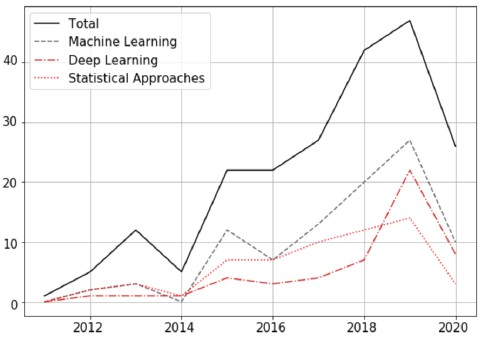
\includegraphics[width=10cm]{assets/literature-review/num-of-anomaly-detection-papers.jpg}
    \caption{Number of papers published work on anomaly detection in cloud computing environments \citep{hagemann2020systematic}}
    \label{fig:num-of-anomaly-detection-paperss}
\end{figure}

\subsubsection{Standard machine learning}

\cite{du2018anomaly} tried experimenting on four of the most popular machine learning techniques to detect performance anomalies. To do this they used an open-source virtual IP Multimedia subsystem called Clearwater. Their system had three modules monitoring agent, data processing, and fault injector. To run the experiment they first used a load generator to create traffic inside the system. Then they used the monitoring agent to collect telemetry data while the fault injector is introducing random faults to the system. Finally, they combined the data from the monitoring agent and the fault injector to create the dataset to train four machine learning models. After training each model was a plugin to the data processing module and tested its precision, recall, and f1-score. In the end, they concluded K Nearest Neighbors classifier gives the most accurate classifications while Support vector machines have the worse.


\subsubsection{Encoder-decoder networks}

\textbf{Auto-encoder}

Auto-encoders are a type of neural network that will try to predict the input data from itself. To do that model has to learn a way to pass through the input data to the output layer through a bottleneck layer. After training this bottleneck layer is called latent space which compressed low-level representation of the entire input data distribution \citep{hinton2006reducing}. So the job of the autoencoder is to understand the underlying pattern in the given data distribution.

Due to this nature, autoencoders have become a popular method of detecting anomalies in time series data since to find anomalies from input sequence one has to learn to identify normal and the abnormal. After training the model on the target dataset, it should be able to come up with the generalized function about the given dataset and it will be able to recreate any input sequence accurately. However, when there is an anomaly in the input sequence models, the output will be vastly different from the input because the model doesn't know how to recreate it properly. This reconstruction loss can be used as a metric to uncover anomalies within the system. In \cite{kumarage2018anomaly} authors used this method to detect anomalies in distributed systems. The main benefit for this approach dataset doesn't have to be labeled and the model learn to differentiate normal from the abnormal.

\textbf{Generative adversarial networks}

In a continuation of their work \cite{kumarage2019generative} they tried doing the same thing but in the opposite way using a \ac{gan} \citep{goodfellow2014generative}. Here the generator network tries to learn the target data distribution (non-anomalous dataset) while the discriminator is trying to classify the normal and abnormal. In this, the generator network acts as the decoder while the discriminator network tries to encode the generator's output into a single scalar value which is the anomaly score. Authors of the paper tried using a traditional \ac{gan} and Bidirectional Generative Adversarial Network (BiGAN) \citep{donahue2016adversarial} but in the end, they concluded even though it showed a tendency towards better performance when the dataset gets bigger, with the dataset they had autoencoders perform well overall.

\subsubsection{Convolutional neural networks}

Ever since DeepMind came up with wavenet which used a CNN to generate audio samples \citep{oord2016wavenet} researchers uncovered other potential use cases other than image-related tasks. One of those use cases was as CNN excels at pattern recognition, encoding time series data set into image-like data structures and using a CNN to identify abnormal patterns in it. On \cite{kim2018encoding} authors tried to use a novel technique to raw encode data into a pixel-like structure and found it could outperform the existing methods to detect anomalies in computer networks. In another work by \cite{zhang2019deep} Convolutional Long-Short Term Memory (ConvLSTM) with an attention mechanism which yielded temporal dependencies more accurately. 


\subsubsection{Root Cause Identification}

Predicting the exact root cause of failure just using a standard machine learning model is a pretty difficult task since prediction space is not finite. In 2017 a team from Google X tried using the Bayesian Network to model the relationship between the state of the system and its effect on failures \citep{chigurupati2017root}. Using it they were able to accurately predict all the possible root causes of a hardware failure in certain systems but this model required to predefine all the possible error modes by domain experts which isn't possible in a constantly evolving distributed system. There were similar attempts \cite{gonzalez2017root} to use machine learning to generate knowledge graphs on historical data and help developers come up with reasoning to failures although this eliminated a need for a domain expert, this also can't react to unseen errors.

In a distributed system it's hard to spot real anomalies just by looking at monitoring data, but when there are huge spikes in response latencies or error rates it's a good indicator something must be wrong. So \cite{samir2019dla} used a \ac{hhmm} to uncover the possible affected services from changes in response time or error rates in one service and used that data to uncover the root cause of the issue. All of the papers discussed above have one problem in common they all assume the entire system is static but in reality, these services changes over time either with increased demand or new future implementations. To address this, \cite{wu2020microrca} developed a service that monitors all the running applications and their vitals. This also constructs an attributed graph that represents how each service interacts with the other. When the monitoring system detects an anomaly MicroRCA weight that graph with response time changes and tries to find the epicenter of the anomaly. The main problem with both of these approaches have is authors rely solely on slow response time as an indication of an anomaly but several other factors could course anomalous behaviors without changes in response times.

\subsection{Comparison of Existing Systems}

\begin{longtable}{| p{25mm} | p{62mm} | p{62mm} |}
\hline
    \textbf{Research} &
    \textbf{Improvements} &
    \textbf{Citations} \\ \hline
    
    \multicolumn{3}{|c|}{\textbf{Instrumentation}} \\ \hline
    
    \cite{toka2021predicting} &
    \vspace{-8mm}
    \begin{itemize}[leftmargin=3mm,noitemsep,nolistsep] 
        \item Explained a way to build a cloud-native data aggregation and analytics pipeline using open-source software.
        \item The proposed system is not platform dependant.
        \vspace{-7mm}
    \end{itemize} &
    \vspace{-8mm}
    \begin{itemize}[leftmargin=3mm,noitemsep,nolistsep] 
        \item The overhead on the monitoring system is a bit high.
        \item Analytics pipelines rely solely on KPI correlation.
        \vspace{-7mm}
    \end{itemize} \\ \hline



    \multicolumn{3}{|c|}{\textbf{Anomaly detection}} \\ \hline
    
    \cite{prabodha2017monitoring} &
    \vspace{-8mm}
    \begin{itemize}[leftmargin=3mm,noitemsep,nolistsep] 
        \item Explained the most popular methods to detect anomalies.
        \vspace{-7mm}
    \end{itemize} &
    \vspace{-8mm}
    \begin{itemize}[leftmargin=3mm,noitemsep,nolistsep] 
        \item The authors didn't consider learning-based approaches.
        \vspace{-7mm}
    \end{itemize} \\ \hline
    
    \cite{kumarage2018anomaly} &
    \vspace{-8mm}
    \begin{itemize}[leftmargin=3mm,noitemsep,nolistsep] 
        \item Due to the difficulty of finding labeled research data, they settled on using a semi-supervised technique.
        \item Used randomized decision trees were utilized to select the most suitable features that correspond to each component.
        \vspace{-7mm}
    \end{itemize} &
    \vspace{-8mm}
    \begin{itemize}[leftmargin=3mm,noitemsep,nolistsep] 
        \item The model won't be easily transformable for other systems.
        \item If more new key features were added to the system it will require total retraining.
        \vspace{-7mm}
    \end{itemize} \\ \hline
    
    \cite{kim2018encoding} &
    \vspace{-8mm}
    \begin{itemize}[leftmargin=3mm,noitemsep,nolistsep] 
        \item Introduced a new encoding technique so CNN can identify anomalies better.
        \vspace{-7mm}
    \end{itemize} &
    \vspace{-8mm}
    \begin{itemize}[leftmargin=3mm,noitemsep,nolistsep] 
        \item Even though this outperformed the “gray-scale encoding” \citep{dasgupta2002anomaly} technique, a comparison study with random forest showed this method gets outperformed by random forest.
        \vspace{-7mm}
    \end{itemize} \\ \hline
    
    \cite{du2018anomaly} &
    \vspace{-8mm}
    \begin{itemize}[leftmargin=3mm,noitemsep,nolistsep] 
        \item Introduced SLIs to monitor data.
        \item A lot of good metrics (input data).
        \item Performance monitoring of services and containers.
        \item Tested multiple Machine learning models to see which one works best.
        \item Introduce a Fault Injection System.
        \vspace{-7mm}
    \end{itemize} &
    \vspace{-8mm}
    \begin{itemize}[leftmargin=3mm,noitemsep,nolistsep] 
        \item Only can identify predetermined issues.
        \item Require a sidecar that includes a lot of overhead.
        \item Won't work with event-driven architectures.
        \item Uses Supervised learning and it's near impossible to find real-world data with labels.
        \vspace{-7mm}
    \end{itemize} \\ \hline
    
    \cite{kumarage2019generative} &
    \vspace{-8mm}
    \begin{itemize}[leftmargin=3mm,noitemsep,nolistsep] 
        \item Used a different approach to predict the future timesteps from the past events.
        \item Which outperformed passed techniques when the monitored data points become larger.
        \vspace{-7mm}
    \end{itemize} &
    \vspace{-8mm}
    \begin{itemize}[leftmargin=3mm,noitemsep,nolistsep] 
        \item Accuracy is around 60\% which is not good to use in production with mission-critical systems.
        \item As this is a GAN-based system, it may take a lot of resources to run with production systems.
        \vspace{-7mm}
    \end{itemize} \\ \hline
    
    \cite{zhang2019deep} &
    \vspace{-8mm}
    \begin{itemize}[leftmargin=3mm,noitemsep,nolistsep] 
        \item Introduce a new embedding technique.
        \item A used hybrid method which uses convolutional autoencoder and LSTM network.
        \vspace{-7mm}
    \end{itemize} &
    \vspace{-8mm}
    \begin{itemize}[leftmargin=3mm,noitemsep,nolistsep] 
        \item Feature maps aren't iterative to understand so operators have to blindly trust the network.
        \item It will be hard to set the network to ignore expected anomalies.
        \vspace{-7mm}
    \end{itemize} \\ \hline
    
    
    \multicolumn{3}{|c|}{\textbf{Root cause identification}} \\ \hline
        
    \cite{chigurupati2017root} &
    \vspace{-8mm}
    \begin{itemize}[leftmargin=3mm,noitemsep,nolistsep] 
        \item Experimented with different metrics till it narrowed down.
        \item Find hidden meaning in values that seems random.
        \item Used a probabilistic approach to better understand the relationship between inputs and outputs.
        \item Gives all the possible root causes of a given problem.
        \vspace{-7mm}
    \end{itemize} &
    \vspace{-8mm}
    \begin{itemize}[leftmargin=3mm,noitemsep,nolistsep] 
        \item Require support from domain experts.
        \item Can't account for unforeseen error.
        \vspace{-7mm}
    \end{itemize} \\ \hline
    
    \cite{gonzalez2017root} &
    \vspace{-8mm}
    \begin{itemize}[leftmargin=3mm,noitemsep,nolistsep] 
        \item Build a predictable system.
        \item Automatic identification of dependencies between system events.
        \item Doesn't Need to rely on Domain experts.
        \item Generalized to different systems.
        \item Used data windowing.
        \item Randomly permuting to test how the model reacts to random inputs.
        \vspace{-7mm}
    \end{itemize} &
    \vspace{-8mm}
    \begin{itemize}[leftmargin=3mm,noitemsep,nolistsep] 
        \item The knowledge graph is good for visualization of the problem but still, people have to manually figure out what went wrong.
        \item It assumes that the collaboration and knowledge of network operators and managers are available.
        \item Random Forests doesn't scale well for a big input set.
        \vspace{-7mm}
    \end{itemize} \\ \hline
    
    \cite{samir2019dla} &
    \vspace{-8mm}
    \begin{itemize}[leftmargin=3mm,noitemsep,nolistsep] 
        \item Custom HHMM model.
        \item Self-healing mechanism.
        \item Focus on performance detection and identification at the container, node, and microservice level.
        \vspace{-7mm}
    \end{itemize} &
    \vspace{-8mm}
    \begin{itemize}[leftmargin=3mm,noitemsep,nolistsep] 
        \item The input dataset scale is limited.
        \item Require a sidecar.
        \item Needs predetermined thresholds.
        \vspace{-7mm}
    \end{itemize} \\ \hline
    
    \cite{wu2020microrca} &
    \vspace{-8mm}
    \begin{itemize}[leftmargin=3mm,noitemsep,nolistsep] 
        \item Created a custom Faults Injection module.
        \item Uses an attribute graph to localize to faulty service.
        \item Application-agnostic by using a service mesh.
        \item Rely on service mesh to determine network topology.
        \item Used Unsupervised learning.
        \vspace{-7mm}
    \end{itemize} &
    \vspace{-8mm}
    \begin{itemize}[leftmargin=3mm,noitemsep,nolistsep] 
        \item Only able to identify 3 types of issues.
        \item Looks only for performance anomalies.
        \item Use the slow response time of a microservice as the definition of an anomaly.
        \item Service meshes add a lot of overhead to systems.
        \item Paper doesn't talk about services that ain't directly connected.
        \item Won't work with event-driven architectures.
        \vspace{-7mm}
    \end{itemize} \\ \hline
    
    \caption{Review of existing systems (self-composed)}
\end{longtable}


\subsection{Benchmark}
Since both \ac{aiops} and automated root cause analysis emerging fields  there isn't any standard way to benchmark the system against the existing ones. So the author is hoping to perform a baseline benchmark with all the existing work based on a few key metrics like f1-score and memory footprint of the system.